%\documentclass[a4paper,landscape, 5pt]{article}
\documentclass[10pt]{article}
\usepackage[a4paper, margin=0.1in, landscape]{geometry}
%\usepackage{graphicx} % Required for inserting images
\usepackage{graphicx}
\usepackage{multicol}
\usepackage{xcolor}
\usepackage{amsfonts}
\usepackage{wrapfig}
\usepackage{amsmath}  % For various math symbols and 
\usepackage{amssymb}  % For additional math symbols
\usepackage{bm}       % For bold math symbols

\usepackage{lipsum}

\usepackage[compact]{titlesec}
% Change title spacing
\titlespacing{\section}{0pt}{*0}{*0}
\titlespacing{\subsection}{0pt}{*0}{*0}
\titlespacing{\subsubsection}{0pt}{*0}{*0}

% Change title color
% \newcommand{\sectionnewcolor}[1]{%
%     \definecolor{section_color}{rgb}{#1}%
%     \titleformat*{\section}{\normalfont\normalsize\bfseries\color{section_color}}%
%     \titleformat*{\subsection}{\normalfont\normalsize\bfseries\color{section_color}}%
%     \titleformat*{\subsubsection}{\normalfont\normalsize\bfseries\color{section_color}}%
% }
\definecolor{default_section_color}{rgb}{0,0,0} % Default color
\newcounter{colornumber}
\setcounter{colornumber}{1}
\newcommand{\sectionnewcolor}{%
    \ifcase\thecolornumber%
        \colorlet{section_color}{red}%
    \or
        \colorlet{section_color}{green}%
    \or
        \colorlet{section_color}{blue}%
    \or
        \colorlet{section_color}{cyan}%
    \or
        \colorlet{section_color}{magenta}%
    \or
        \colorlet{section_color}{yellow}%
    \or
        \colorlet{section_color}{orange}%
    \or
        \colorlet{section_color}{purple}%
    \or
        \colorlet{section_color}{teal}%
    \or
        \colorlet{section_color}{lime}%
    \or
        \colorlet{section_color}{pink}%
    \or
        \colorlet{section_color}{brown}%
    \or
        \colorlet{section_color}{indigo}%
    \or
        \colorlet{section_color}{turquoise}%
    \or
        \colorlet{section_color}{gold}%
    \or
        \colorlet{section_color}{silver}%
    \or
        \colorlet{section_color}{slategray}%
    \or
        \colorlet{section_color}{olive}%
    \or
        \colorlet{section_color}{maroon}%
    \else
        \colorlet{section_color}{default_section_color}%
    \fi
    
    \titleformat*{\section}{\normalfont\normalsize\bfseries\color{section_color}}%
    \titleformat*{\subsection}{\normalfont\normalsize\bfseries\color{section_color}}%
    \titleformat*{\subsubsection}{\normalfont\normalsize\bfseries\color{section_color}}%
    \stepcounter{colornumber}%
}

\newcommand{\sectiondivider}{%
    \vspace{4pt}%
    \hrule%
    \vspace{4pt}%
}

% Change text spacing
\setlength{\parindent}{0pt}
\setlength{\columnseprule}{0.2pt}
\setlength{\intextsep}{0pt}%
% \setlength{\columnsep}{7pt}%

\begin{document}

\begin{multicols*}{4}

\sectionnewcolor
\section*{Regression}
\subsection*{Terminology}

- Data consists of \textbf{pairs} ($\mathbf{x}_n$, $y_n$), where $y_n$ is the n’th output and $x_n$ is a vector of $D$ inputs. The number of pairs $N$ is the data-size and $D$ is the dimensionality.

- Two goals of regression: \textbf{prediction} and \textbf{interpretation}

- The regression function: $y_{n}\approx f_w(\mathbf{x}_{n})\ \forall n$

- Regression finds correlation not a causal relationship.

- \textbf{Input variables} a.k.a. covariates, independent variables, explanatory variables, exogenous variables, predictors, regressors. 

- \textbf{Output variables} a.k.a. target, label, response, outcome, dependent variable, endogenous variables, measured variable, regressands.

\subsection*{Linear Regression}

- Assumes linear relationship between inputs and output.

- $y_{n}\approx\,f(\mathbf{x}_{n}) :=w_{0}+w_{1}x_{n1}+ ... +w_{D}x_{n D} \\ := \tilde{\bf x}_{n}^{T} \tilde{\bf w}$ contain the additional offset term (\small{a.k.a. bias}).

- Given data we learn the weights $\mathbf{w}$ (\small{a.k.a. estimate or fit the model})

- Overparameterisation $D > N$ eg. univariate linear regression with a single data point $y_{1}\approx w_{0}+w_{1}x_{11}$. This makes the task under-determined (no unique solution).

\subsection*{Loss Functions $\mathcal{L}$}

- A loss function (a.k.a. energy, cost, training objective) quantifies how well the model does (how costly its mistakes are).

- $y \in \mathbb{R} \Rightarrow$ desirable for cost to be symmetric around 0 since $\pm$ errors should be penalized equally.

- Cost function should penalize “large” mistakes and “very large” mistakes similarly to be robust to outliars.

- Mean Squared Error: \\ ${\mathsf{MSE}}(\mathbf{w}):={\frac{1}{N}}\sum_{n=1}^{N}\left[y_{n}-f_{\mathrm{w}}(\mathbf{x}_{n})\right]^{2}$ \\ not robust to outliars.

- Mean Absolute Error: \\ ${\mathsf{MAE}}(\mathbf{w}):={\frac{1}{N}}\sum_{n=1}^{N}|y_{n}-f_{\mathrm{w}}(\mathbf{x}_{n})|$

- Convexity: a function is convex iff a line segment between two points on the function’s graph always lies above the function.

- Convexity: a function $h(\mathbf{u}), \mathbf{u} \in \mathbb{R}^D$ is convex if $\forall \ \mathbf{u}, \mathbf{v} \in \mathbb{R}^D, 0 \leq \lambda \leq  1$: \\ $h(\lambda\mathbf{u}+(1-\lambda)\mathbf{v}) \ \textcolor[RGB]{255,0,0}{\leq} \ \lambda h(\mathbf{u})+(1-\lambda)h(\mathbf{v})$ \\Stirctly convex if $\textcolor[RGB]{255,0,0}{\leq} \Rightarrow \textcolor[RGB]{255,0,0}{<}$ 

- Convexity, a desired computational property:
A strictly convex function has a unique global minimum $\mathbf{w^{*}}$. For convex functions, every local minimum is a global minimum.

- Sums of convex functions are also convex $\Rightarrow$ MSE combined with a linear model is convex in $\mathbf{w}$.

- Proof of convexity for MAE:

\scalebox{0.7}{
$\begin{array}{l}
    {\mathsf{MAE}(\mathbf{w}) := \frac{1}{N} \sum_{n=1}^{N} \mathcal{L}_n(\mathbf{w}), \mathcal{L}_n(\mathbf{w})=|y_{n}-f_{\mathrm{w}}(\mathbf{x}_{n})|} 
    \\ 
    {\mathcal{L}_n(\lambda w_1 + (1-\lambda)w_2) \leq \lambda \mathcal{L}_n(w_1)+(1-\lambda)\mathcal{L}_n(w_2)} 
    \\ 
    {| y_n-x_n^{T}(\lambda w_1 + (1-\lambda)w_2)| \leq \lambda |{y_n-x_n^{T}w_1}| + (1-\lambda)|{y_n-x_n^{T}w_2}|}
    \\
    {(1-\lambda) \geq 0 \Rightarrow (1-\lambda)|{y_n-x_n^{T}w_2}|=|(1-\lambda)y_{n}-(1-\lambda)x_{n}^{T}w_2|}
    \\
    {a=\lambda y_{n}-\lambda x_{n}^{T}w_{1}, b=(1-\lambda)y_{n}-(1-\lambda)x_{n}^{T}w_{2}}
    \\
    {a+b=y_{n}-x_{n}^{T}(\lambda w_{1}+(1-\lambda)w_{2})}
    \\
    {|a + b| \leq |a| + |b| \Rightarrow \mathcal{L}_n(\mathbf{w}) \ \mathsf{convex}\Rightarrow \mathsf{MAE}(\mathbf{w}) \ \mathsf{convex}}
\end{array}$
}

- Huber loss: \\
${\cal H}u b e r(e):=\left\{\begin{array}{l l}{{\frac{1}{2}e^{2}}}&{{,\mathrm{if}\ |e|\leq\delta}}\\ {{\delta|e|-\frac{1}{2}\delta^{2}}}&{{,\mathrm{if}\ |e|>\delta}}\end{array}\right.$ convex, differentiable, and robust to outliers but setting $\delta$ is not easy.

- Tukey’s bisquare loss: \\
$\frac{\partial\mathcal{L}}{\partial e}:=\left\{\begin{array}{l l}{{e\{1-e^{2}/\delta^{2}\}^{2}}}&{{,\mathrm{if}\,\,|e|\leq\delta}}\\ {{0}}&{{,\mathrm{if} \ |e| > \delta}}\end{array}\right.$ non-convex, but robust to outliers.

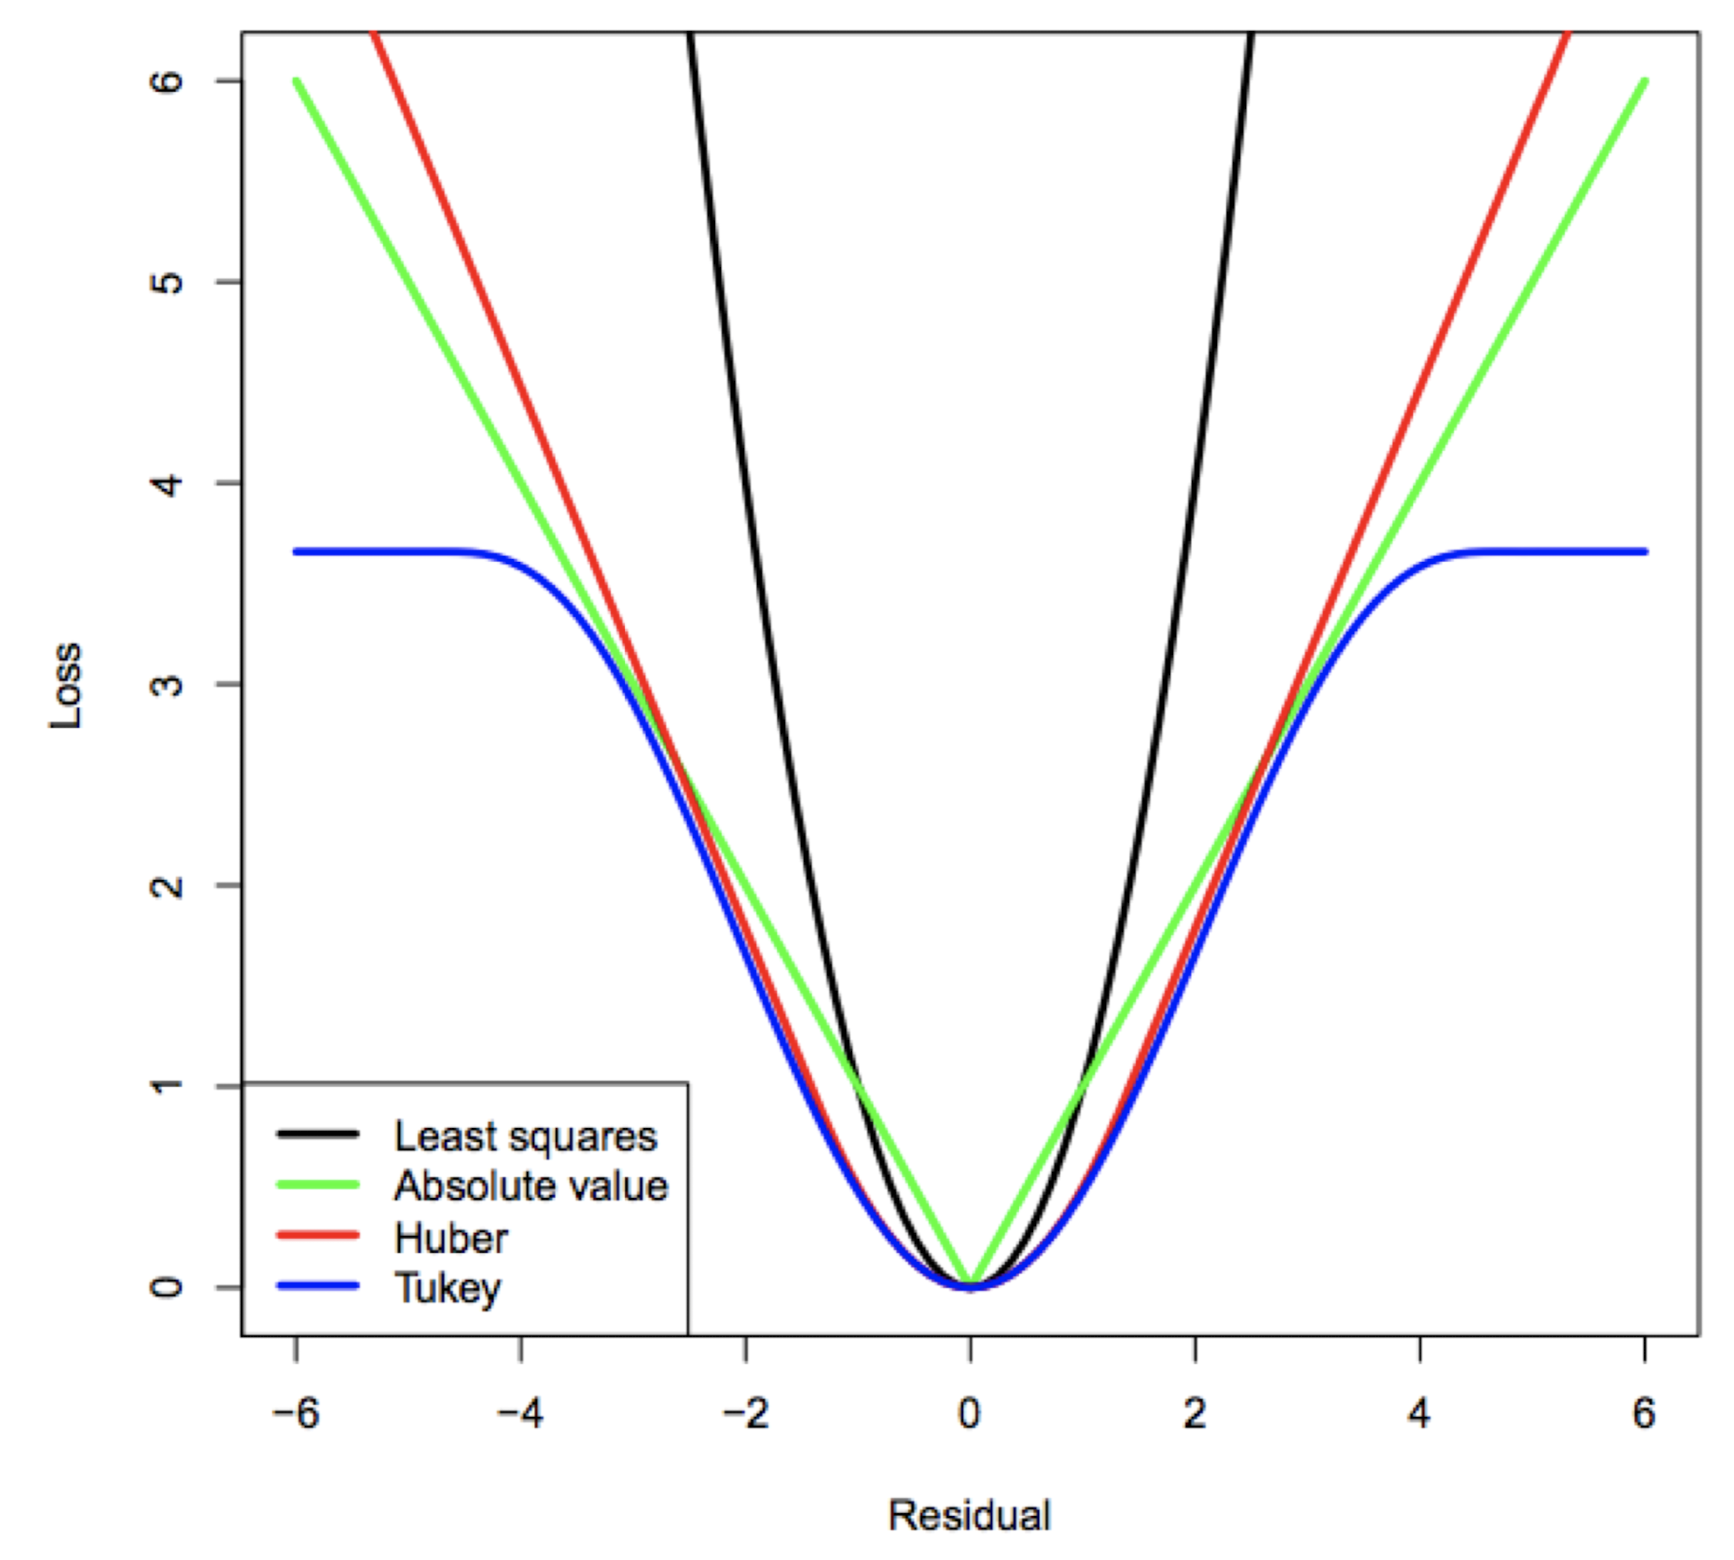
\includegraphics[width=\linewidth]{loss_functions.png}
\sectiondivider

\sectionnewcolor
\section{Optimisation}

- Given $\mathcal{L}(\mathbf{w})$ we want $\mathbf{w^*} \in \mathbb{R}^D$ which minimises the cost: $\min_\mathbf{w} \mathcal{L}(\mathbf{w}) \rightarrow$ formulated as an optimisation problem

- Local minimum $\mathbf{w^*} \Rightarrow \exists \epsilon > 0$ s.t. \\
$\mathcal{L}(\mathbf{w^*}) \leq \mathcal{L}(\mathbf{w}) \ \forall \mathbf{w} \ \mathrm{with} \ \Vert \mathbf{w}-\mathbf{w^*} \Vert < \epsilon$

- Global minimum $\mathbf{w^*}$,
$\mathcal{L}(\mathbf{w^*}) \leq \mathcal{L}(\mathbf{w}) \ \forall \mathbf{w} \in \mathbb{R}^D$

\subsection{Smooth Optimisation}

\vspace{4pt}
\hrule
\vspace{4pt}
\sectiondivider

\sectionnewcolor

\section*{Least Squares}
- Linear regression + MSE $\rightarrow$ compute the optimum of the cost function analytically by solving a linear system of $D$ equations (normal equations)

- Derive the normal equations, proove convexity, optimality conditions for convex functions ($
\nabla \mathcal{L}\left(\mathbf{w}^{\star}\right)=\mathbf{0} .
$)

\subsection*{Normal Equations}
$\mathcal{L}(\mathbf{w})=\frac{1}{2 N} \sum_{n=1}^{N}\left(y_{n}-\mathbf{x}_{n}^{\top} \mathbf{w}\right)^{2}\\=\frac{1}{2 N}(\mathbf{y}-\mathbf{X} \mathbf{w})^{\top}(\mathbf{y}-\mathbf{X} \mathbf{w})$,

% where

% $\mathbf{y}=\left[\begin{array}{c}y_{1} \\ y_{2} \\ \vdots \\ y_{N}\end{array}\right], \mathbf{X}=\left[\begin{array}{cccc}x_{11} & x_{12} & \ldots & x_{1 D} \\ x_{21} & x_{22} & \ldots & x_{2 D} \\ \vdots & \vdots & \ddots & \vdots \\ x_{N 1} & x_{N 2} & \ldots & x_{N D}\end{array}\right]$

- Proof of convexity:

1) Simplest way: observe that $\mathcal{L}$ is naturally represented as the sum (with positive coefficients) of the simple terms $\left(y_{n}-\mathbf{x}_{n}^{\top} \mathbf{w}\right)^{2}$. Further, each of these simple terms is the composition of a linear function with a convex function (the square function). Therefore, each of these simple terms is convex and hence the sum is convex.

2) Directly verify the definition, that for any $\lambda \in[0,1]$ and $\mathbf{w}, \mathbf{w}^{\prime}$

\text{\footnotesize
$\mathcal{L}\left(\lambda \mathbf{w}+(1-\lambda) \mathbf{w}^{\prime}\right)-\left(\lambda \mathcal{L}(\mathbf{w})+(1-\lambda) \mathcal{L}\left(\mathbf{w}^{\prime}\right)\right) \leq 0$.
}

$\mathrm{LHS}=$
$-\frac{1}{2 N} \lambda(1-\lambda)\left\|\mathbf{X}\left(\mathbf{w}-\mathbf{w}^{\prime}\right)\right\|_{2}^{2} < 0$,


3) We can compute the second derivative (the Hessian) and show that it is positive semidefinite (all its eigenvalues are non-negative). 

$\begin{aligned}
    \mathbf{H}(\mathbf{w})& =\frac{1}{2N}\nabla^2\left(\left(\mathbf{y}-\mathbf{X}\mathbf{w}\right)^\top\left(\mathbf{y}-\mathbf{X}\mathbf{w}\right)\right)  \\
    &=\frac{1}{2N}\nabla\left(-2(\mathbf{y}-\mathbf{X}\mathbf{w})\mathbf{X}^\top\right) \\
    &=\frac{-2}{2N}\nabla(\mathbf{X}^\top(\mathbf{y}-\mathbf{X}\mathbf{w})) \\
    &=\frac{-1}N\mathbf{X}^\top\nabla(\mathbf{y}-\mathbf{X}\mathbf{w}) \\
    &=\frac{-1}N\mathbf{X}^\top(\nabla\mathbf{y}-\nabla(\mathbf{X}\mathbf{w})) \\
    &=\frac{-1}N\mathbf{X}^\top(\mathbf{0}-\mathbf{X}) \\
    &=\frac1N\mathbf{X}^\top\mathbf{X}
\end{aligned}$

Singular value decomposition (SVD):
$
\mathbf{X}=\mathbf{US}\mathbf{V}^\top 
$
U and V are orthogonal matrices, and S is a diagonal matrix with the singular values $\sigma_i$ on the diagonal.

$
\mathbf{H}(\mathbf{w})=\frac1N\mathbf{X}^\top\mathbf{X}=\frac1N\mathbf{V}\mathbf{S}^2\mathbf{V}^\top 
$

where $\mathbf{S}^2$ is a diagonal matrix with the squares of the singular values. 

Let $\mathbf{v}$ be a non-zero vector,

$
\begin{aligned}
\mathbf{v}^\top\mathbf{H}(\mathbf{w})\mathbf{v}& =\frac1N\mathbf{v}^\top\mathbf{V}\mathbf{S}^2\mathbf{V}^\top\mathbf{v} \\
&=\frac1N(\mathbf{V}^\top\mathbf{v})^\top\mathbf{S}^2(\mathbf{V}^\top\mathbf{v}) \\
&=\frac1N\|\mathbf{S}(\mathbf{V}^\top\mathbf{v})\|^2 \geq 0
\end{aligned}
$

$\mathbf{S}$ diagonal matrix with non-negative entries, $\mathbf{V}^\top\mathbf{v}$ vector.


- Now find its minimum

$
\nabla \mathcal{L}(\mathbf{w})=-\frac{1}{N} \mathbf{X}^{\top}(\mathbf{y}-\mathbf{X} \mathbf{w}) = \mathbf{0}\\
\Rightarrow\mathbf{X}^{\top} \underbrace{(\mathbf{y}-\mathbf{X} \mathbf{w})}_{\text {error }}=\mathbf{0}
$

\subsection*{Geometric Interpretation}

% \begin{center}
    \includegraphics*[width=0.7\columnwidth]{figures/geom_ls.png}
% \end{center}


\subsection*{Closed form}
- $\mathbf{X}^{\top} \mathbf{X} \in \mathbb{R}^{D \times D}$ is called the Gram matrix. 

- If invertible, we can get a closed-form expression for the minimum:

$
\mathbf{w}^{\star}=\left(\mathbf{X}^{\top} \mathbf{X}\right)^{-1} \mathbf{X}^{\top} \mathbf{y}
$

\subsection*{Invertibility and Uniqueness}
- $\mathbf{X}^{\top} \mathbf{X} \in \mathbb{R}^{D \times D}$ invertible iff $\operatorname{rank}(\mathbf{X})=D$.

- Proof: assume $\operatorname{rank}(\mathbf{X})<D$. Then there exists a non-zero vector $\mathbf{u}$ so that $\mathbf{X u}=\mathbf{0}$. It follows that $\mathbf{X}^{\top} \mathbf{X u}=\mathbf{0}$, and so $\operatorname{rank}\left(\mathbf{X}^{\top} \mathbf{X}\right)<D$. Therefore, $\mathbf{X}^{\top} \mathbf{X}$ is not invertible.

Conversely, assume that $\mathbf{X}^{\top} \mathbf{X}$ is not invertible. Hence, there exists a non-zero vector $\mathbf{v}$ so that $\mathbf{X}^{\top} \mathbf{X v}=\mathbf{0}$. It follows that

$$
\mathbf{0}=\mathbf{v}^{\top} \mathbf{X}^{\top} \mathbf{X} \mathbf{v}=(\mathbf{X} \mathbf{v})^{\top}(\mathbf{X} \mathbf{v})=\|\mathbf{X} \mathbf{v}\|^{2}
$$

This implies that $\mathbf{X v}=\mathbf{0}$, i.e., $\operatorname{rank}(\mathbf{X})<D$.

\subsection*{Rank Deficiency and Ill-Conditioning}
- In practice, $\mathbf{X}$ is often rank deficient.

- If $D>N$, we always have $\operatorname{rank}(\mathbf{X})<D$ (since row rank $=$ col. rank)

- If $D \leq N$, but some of the columns $\mathbf{x}_{:}$are (nearly) collinear, then the matrix is illconditioned, leading to numerical issues when solving the linear system.

- Using a linear system solver, one can solve this problem.

\subsection*{Closed-form solution for MAE}
Can you derive closed-form solution for 1-parameter model when using MAE cost function?


\sectiondivider

\sectionnewcolor

\section*{Overfitting}
Models can be too limited or they can be too rich. In the first case we cannot find a function that is a good fit for the data in our model. We then say that we underfit. In the second case we have such a rich model family that we do not just fit the underlying function but we in fact fit the noise in the data as well. We then talk about an overfit. Both of these phenomena are undesirable. This discussion is made more difficult since all we have is data and so we do not know a priori what part is the underlying signal and what part is noise.

\section*{Underfitting with Linear Models}
It is easy to see that linear models might underfit. Consider a scalar case as shown in the figure below.


The solid curve is the underlying function and the circles are the actual data. E.g., we assume that there is a scalar function $g(x)$ but that we do not observe $g\left(x_{n}\right)$ directly but only a noisy version of it, $y_{n}=g\left(x_{n}\right)+Z_{n}$, where $Z_{n}$ is
the noise. The noise might be due for example to some measurement inaccuracies. The $y_{n}$ are shown as blue cirles. If our model family consists of only linear functions of the scalar input $x$, i.e., $\mathcal{F}=\left\{f_{w}(x)=w x\right\}$, where $w$ is a scalar constant (the slope of the function), then it is clear that we cannot match the given function accurately, regardless how many samples we get and how small the noise is. We therefore will underfit.

Extended/Augmented Feature Vectors From the above example it might seem that linear models are too simple to ever overfit. But in fact, linear models are highly prone to overfitting, much more so than complicated models like neural nets.

Since linear models are inherently not very rich the following is a standard "trick" to make them more powerful.

In order to increase the representational power of linear models we typically "augment" the input. E.g., if the input (feature) is one-dimensional we might add a polynomial basis (of arbitrary degree $M$ ),

$$
\boldsymbol{\phi}\left(x_{n}\right):=\left[1, x_{n}, x_{n}^{2}, x_{n}^{3}, \ldots, x_{n}^{M}\right]
$$

so that we end up with an extended feature vector.

We then fit a linear model to this extended feature vector $\phi\left(x_{n}\right)$ :

$$
y_{n} \approx w_{0}+w_{1} x_{n}+w_{2} x_{n}^{2}+\ldots+w_{M} x_{n}^{M}=: \boldsymbol{\phi}\left(x_{n}\right)^{\top} \mathbf{w}
$$

\section*{Overfitting with Linear Models}
In the following four figures, circles are data points, the green line represents the "true function", and the red line is the model. The parameter $M$ is the maximum degree in the polynomial basis.

For $M=0$ (the model is a constant) the model is underfitting and the same is true for $M=1$. For $M=3$ the model fits the data fairly well and is not yet so rich as to fit in addition the small "wiggles" caused by the noise. But for $M=9$ we now have such a rich model that it can fit every single data point and we see severe overfitting taking place. What can we do to avoid overfitting? If you increase the amount of data (increase $N$, but keep $M$ fixed), overfitting
might reduce. This is shown in the following two figures where we again consider the same model complexity $M=9$ but we have extra data $(N=15$ or even $N=100)$.

\section*{A Word About Notation}
If it is important to distinguish the original input $\mathbf{x}$ from the augmented input then we will use $\phi(\mathbf{x})$ to denote this augmented input vector. But we can consider this augmentation as part of the pre-processing, and then we might simply write $\mathbf{x}$ to denote the input. This will save us a lot of notation.

\section*{Additional Materials}
Read about overfitting in the paper by Pedro Domingos (Sections 3 and 5 of "A few useful things to know about machine learning").

\sectiondivider

\sectionnewcolor
\section{Maximum Likelihood}

\subsection*{Gaussian distribution and independence}
% - A Gaussian random variable in $\mathbb{R}$ with mean $\mu$ and variance $\sigma^{2}$ has a density of

$p(y \mid \mu, \sigma^{2})=\mathcal{N}(y \mid \mu, \sigma^{2})=\frac{1}{\sqrt{2 \pi \sigma^{2}}} \exp [-\frac{(y-\mu)^{2}}{2 \sigma^{2}}]$,
$\boldsymbol{\Sigma}$ psd.

$\mathcal{N}(\mathbf{y} \mid \boldsymbol{\mu}, \boldsymbol{\Sigma})=\frac{1}{\sqrt{(2 \pi)^{D} \operatorname{det}(\boldsymbol{\Sigma})}} \exp [-\frac{1}{2}(\mathbf{y}-\boldsymbol{\mu})^{\top} \boldsymbol{\Sigma}^{-1}(\mathbf{y}-\boldsymbol{\mu})]$

- Two RVs $X$, $Y$ independent when $p(x, y)=p(x) p(y)$.

\subsection*{A probabilistic model for least-squares}

- $
y_{n}=\mathbf{x}_{n}^{\top} \mathbf{w}+\epsilon_{n}
$ where the $\epsilon_{n}$ zero mean Gaussian RV

% - Given $N$ samples, the likelihood of the data vector $\mathbf{y}=$ $(y_{1}, \cdots, y_{N})$ given the input $\mathbf{X}$ and the model $\mathbf{w}$ is equal to

$p(\mathbf{y} \mid \mathbf{X}, \mathbf{w})=\prod_{n=1}^{N} p(y_{n} \mid \mathbf{x}_{n}, \mathbf{w})=\prod_{n=1}^{N} \mathcal{N}(y_{n} \mid \mathbf{x}_{n}^{\top} \mathbf{w}, \sigma^{2})$

% - Maximize this likelihood over the choice of model w.

\subsection*{Defining cost with log-likelihood}

$\mathcal{L}_{\mathrm{LL}}(\mathbf{w}):=\log p(\mathbf{y} \mid \mathbf{X}, \mathbf{w})=-\frac{1}{2 \sigma^{2}} \sum_{n=1}^{N}(y_{n}-\mathbf{x}_{n}^{\top} \mathbf{w})^{2}+$ cnst.

\subsection*{Maximum-likelihood estimator (MLE)}

$\arg \min _{\mathbf{w}} \mathcal{L}_{\mathrm{MSE}}(\mathbf{w})=\arg \max _{\mathbf{w}} \mathcal{L}_{\mathrm{LL}}(\mathbf{w})$.

% - MLE $\rightarrow$ finding the model under which the observed data is most likely to have been generated from (probabilistically).

\subsection*{Properties of MLE}
- MLE is a sample approximation to the expected log-likelihood:
$
\mathcal{L}_{\mathrm{LL}}(\mathbf{w}) \approx \mathbb{E}_{p(y, \mathbf{x})}[\log p(y \mid \mathbf{x}, \mathbf{w})]
$

- MLE is consistent, i.e., it will give us the correct model assuming that we have a sufficient amount of data.
$\mathbf{w}_{\text {MLE }} \longrightarrow^{p} \mathbf{w}_{\text {true }}$

- The MLE is asymptotically normal, i.e.,

$(\mathbf{w}_{\text {MLE }}-\mathbf{w}_{\text {true }}) \longrightarrow^{d} \frac{1}{\sqrt{N}} \mathcal{N}(\mathbf{w}_{\text {MLE }} \mid \mathbf{0}, \mathbf{F}^{-1}(\mathbf{w}_{\text {true }}))$

where $\mathbf{F}(\mathbf{w})=-\mathbb{E}_{p(\mathbf{y})}[\frac{\partial^{2} \mathcal{L}}{\partial \mathbf{w} \partial \mathbf{w}^{\top}}]$ is the Fisher information.

- MLE is efficient, i.e. it achieves the Cramer-Rao lower bound. Covariance $(\mathbf{w}_{\text {MLE }})=\mathbf{F}^{-1}(\mathbf{w}_{\text {true }})$

\subsection*{Laplace distribution $
p(y_{n} \mid \mathbf{x}_{n}, \mathbf{w})=\frac{1}{2 b} e^{-\frac{1}{b}|y_{n}-\mathbf{x}_{n}^{\top} \mathbf{w}|}
$}


\sectiondivider

\sectionnewcolor

\section*{Regularization}
We have seen that by augmenting the feature vector we can make linear models as powerful as we want. Unfortunately this leads to the problem of overfitting. Regularization is a way to mitigate this undesirable behavior.

We will discuss regularization in the context of linear models, but the same principle applies also to more complex models such as neural nets.

\section*{Regularization}
Through regularization, we can penalize complex models and favor simpler ones:

$$
\min _{\mathbf{w}} \mathcal{L}(\mathbf{w})+\Omega(\mathbf{w})
$$

The second term $\Omega$ is a regularizer, measuring the complexity of the model given by $\mathbf{w}$.

\section*{$L_{2}$-Regularization: Ridge Regression}
The most frequently used regularizer is the standard Euclidean norm $\left(L_{2^{-}}\right.$ norm), that is

$$
\Omega(\mathbf{w})=\lambda\|\mathbf{w}\|_{2}^{2}
$$

where $\|\mathbf{w}\|_{2}^{2}=\sum_{i} w_{i}^{2}$. Here the main effect is that large model weights $w_{i}$ will be penalized (avoided), since we consider them "unlikely", while small ones are ok. When $\mathcal{L}$ is MSE, this is called ridge regression:

$\min _{\mathbf{w}} \frac{1}{2 N} \sum_{n=1}^{N}\left[y_{n}-\mathbf{x}_{n}^{\top} \mathbf{w}\right]^{2}+\lambda\|\mathbf{w}\|_{2}^{2}$

Least squares is a special case of this: set $\lambda:=0$.

\section*{Explicit solution for w: Differ-}
entiating and setting to zero:

$$
\mathbf{w}_{\text {ridge }}^{\star}=\left(\mathbf{X}^{\top} \mathbf{X}+\lambda^{\prime} \mathbf{I}\right)^{-1} \mathbf{X}^{\top} \mathbf{y}
$$

(here for simpler notation $\frac{\lambda^{\prime}}{2 N}=\lambda$ )

\section*{Ridge Regression to Fight III-Conditioning}
The eigenvalues of $\left(\mathbf{X}^{\top} \mathbf{X}+\lambda^{\prime} \mathbf{I}\right)$ are all at least $\lambda^{\prime}$ and so the inverse always exists. This is also referred to as lifting the eigenvalues.

Proof: Write the Eigenvalue decomposition of $\mathbf{X}^{\top} \mathbf{X}$ as $\mathbf{U S U}^{\top}$. We then have

$$
\begin{aligned}
\mathbf{X}^{\top} \mathbf{X}+\lambda^{\prime} \mathbf{I} & =\mathbf{U S} \mathbf{U}^{\top}+\lambda^{\prime} \mathbf{U I U}^{\top} \\
& =\mathbf{U}\left[\mathbf{S}+\lambda^{\prime} \mathbf{I}\right] \mathbf{U}^{\top}
\end{aligned}
$$

We see now that every Eigenvalue is "lifted" by an amount $\lambda^{\prime}$.

Here is an alternative proof. Recall that for a symmetric matrix $\mathbf{A}$ we can also compute eigenvalues by looking at the so-called Rayleigh ratio,

$$
R(\mathbf{A}, \mathbf{v})=\frac{\mathbf{v}^{\top} \mathbf{A} \mathbf{v}}{\mathbf{v}^{\top} \mathbf{v}}
$$

Note that if $\mathbf{v}$ is an eigenvector with eigenvalue $\lambda$ then the Rayleigh coefficient indeed gives us $\lambda$. We can find the smallest and largest eigenvalue by minimizing and maximizing this coefficient. But note that if we apply this to the symmetric matrix $\mathbf{X}^{\top} \mathbf{X}+\lambda^{\prime} \mathbf{I}$ then for any vector $\mathbf{v}$ we have

$$
\frac{\mathbf{v}^{\top}\left(\mathbf{X}^{\top} \mathbf{X}+\lambda^{\prime} \mathbf{I}\right) \mathbf{v}}{\mathbf{v}^{\top} \mathbf{v}} \geq \frac{\lambda^{\prime} \mathbf{v}^{\top} \mathbf{v}}{\mathbf{v}^{\top} \mathbf{v}}=\lambda^{\prime}
$$

\section*{$L_{1}$-Regularization: The Lasso}
As an alternative measure of the complexity of the model, we can use a different norm. A very important case is the $L_{1}$-norm, leading to $L_{1^{-}}$ regularization. In combination with the MSE cost function, this is known as the Lasso:

$\min _{\mathbf{w}} \frac{1}{2 N} \sum_{n=1}^{N}\left[y_{n}-\mathbf{x}_{n}^{\top} \mathbf{w}\right]^{2}+\lambda\|\mathbf{w}\|_{1}$

where

$$
\|\mathbf{w}\|_{1}:=\sum_{i}\left|w_{i}\right| .
$$


The figure above shows a "ball" of constant $L_{1}$ norm. To keep things simple assume that $\mathbf{X}^{\top} \mathbf{X}$ is invertible. We claim that in this case the set

$$
\left\{\mathbf{w}:\|\mathbf{y}-\mathbf{X} \mathbf{w}\|^{2}=\alpha\right\}
$$

is an ellipsoid and this ellipsoid simply scales around its origin as we change $\alpha$. We claim that for the $L_{1}$-regularization the optimum solution is likely going to be sparse (only has few non-zero components) compared to the case where we use $L_{2}$-regularization.

Why is this the case? Assume that a genie tells you the $L_{1}$ norm of the optimum solution. Draw the $L_{1}$-ball with that norm value (think of $2 \mathrm{D}$ to visualize it). So now you know that the optimal point is somewhere on the surface of this "ball". Further you know that there are ellipsoids, all with the same mean and rotation that describes the equal error surfaces incurred by the first term. The optimum solution is where the "smallest" of these ellipsoids just touches the $L_{1}$-ball. Due to the geometry of this ball this point is more likely to be on one of the "corner" points. In turn, sparsity is desirable, since it leads to a "simple" model.

How do we see the claim that (1) describes and ellipsoid? First look at $\alpha=\|\mathbf{X w}\|^{2}=\mathbf{w}^{\top} \mathbf{X}^{\top} \mathbf{X w}$. This is a quadratic form. Let $\mathbf{A}=\mathbf{X}^{\top} \mathbf{X}$. Note that $\mathbf{A}$ is a symmetric matrix and by assumption it has full rank. If $\mathbf{A}$ is a diagonal matrix with strictly positive elements $a_{i}$ along the diagonal then this describes the equation

$$
\sum_{i} a_{i} \mathbf{w}_{i}^{2}=\alpha
$$

which is indeed the equation for an ellipsoid. In the general case, $\mathbf{A}$ can be written as (using the SVD) $\mathbf{A}=\mathbf{U B U}^{T}$, where $\mathbf{B}$ is a diagonal matrix with strictly positive entries. This then corresponds to an ellipsoid with rotated axes. If we now look at $\alpha=\|\mathbf{y}-\mathbf{X} \mathbf{w}\|^{2}$, where $\mathbf{y}$ is in the column space of $\mathbf{X}$ then we can write it as $\alpha=\left\|\mathbf{X}\left(\mathbf{w}_{0}-\mathbf{w}\right)\right\|^{2}$ for a suitable chosen $\mathbf{w}_{0}$ and so this corresponds to a shifted ellipsoid. Finally, for the general case, write $\mathbf{y}$ as $\mathbf{y}=\mathbf{y}_{\|}+$ $\mathbf{y}_{\perp}$, where $\mathbf{y}_{\|}$is the component of $\mathbf{y}$ that lies in the subspace spanned by the columns of $\mathbf{X}$ and $\mathbf{y}_{\perp}$ is the component that
is orthogonal. In this case

$$
\begin{aligned}
\alpha & =\|\mathbf{y}-\mathbf{X} \mathbf{w}\|^{2} \\
& =\left\|\mathbf{y}_{\|}+\mathbf{y}_{\perp}-\mathbf{X} \mathbf{w}\right\|^{2} \\
& =\left\|\mathbf{y}_{\perp}\right\|^{2}+\left\|\mathbf{y}_{\|}-\mathbf{X} \mathbf{w}\right\|^{2} \\
& =\left\|\mathbf{y}_{\perp}\right\|^{2}+\left\|\mathbf{X}\left(\mathbf{w}_{0}-\mathbf{w}\right)\right\|^{2} .
\end{aligned}
$$

Hence this is then equivalent to the equation $\left\|\mathbf{X}\left(\mathbf{w}_{0}-\mathbf{w}\right)\right\|^{2}=$ $\alpha-\left\|\mathbf{y}_{\perp}\right\|^{2}$, proving the claim. From this we also see that if $\mathbf{X}^{\top} \mathbf{X}$ is not full rank then what we get is not an ellipsoid but a cylinder with an ellipsoidal cross-section.

\section*{Additional Notes}
\section*{Other Types of Regularization}
Popular methods such as shrinkage, dropout and weight decay (in the context of neural networks), early stopping of the optimization are all different forms of regularization.

Another view of regularization: The ridge regression formulation we have seen above is similar to the following constrained problem (for some $\tau>0)$.

$$
\min _{\mathbf{w}} \frac{1}{2 N} \sum_{n=1}^{N}\left(y_{n}-\mathbf{x}_{n}^{\top} \mathbf{w}\right)^{2}, \quad \text { such that }\|\mathbf{w}\|_{2}^{2} \leq \tau
$$

The following picture illustrates this.


Figure 1: Geometric interpretation of Ridge Regression. Blue lines indicating the level sets of the MSE cost function.

For the case of using $L_{1}$ regularization (known as the Lasso, when used with MSE) we analogously consider

$$
\min _{\mathbf{w}} \frac{1}{2 N} \sum_{n=1}^{N}\left(y_{n}-\mathbf{x}_{n}^{\top} \mathbf{w}\right)^{2}, \quad \text { such that }\|\mathbf{w}\|_{1} \leq \tau
$$

This forces some of the elements of $\mathbf{w}$ to be strictly 0 and therefore enforces sparsity in the model (some features will not be used since their coefficients are zero).

\begin{itemize}
  \item Why does $L_{1}$ regularizer enforce sparsity? Hint: Draw the picture similar to above, and locate the optimal solution.
  \item Why is it good to have sparsity in the model? Is it going to be better than least-squares? When and why?
\end{itemize}

\section*{Ridge Regression as MAP estimator}
Recall that classic least-squares linear regression can be interpreted as the maximum likelihood estimator:

$$
\begin{aligned}
& \mathbf{w}_{\mathrm{lse}} \stackrel{(a)}{=} \arg \min _{\mathbf{w}}-\log p(\mathbf{y}, \mathbf{X} \mid \mathbf{w}) \\
& \stackrel{(b)}{=} \arg \min _{\mathbf{w}}-\log p(\mathbf{X} \mid \mathbf{w}) p(\mathbf{y} \mid \mathbf{X}, \mathbf{w}) \\
& \stackrel{(c)}{=} \arg \min _{\mathbf{w}}-\log p(\mathbf{X}) p(\mathbf{y} \mid \mathbf{X}, \mathbf{w}) \\
& \stackrel{(d)}{=} \arg \min _{\mathbf{w}} \quad-\log p(\mathbf{y} \mid \mathbf{X}, \mathbf{w}) \\
& \stackrel{(e)}{=} \arg \min _{\mathbf{w}} \quad-\log \left[\prod_{n=1}^{N} p\left(y_{n} \mid \mathbf{x}_{n}, \mathbf{w}\right)\right] \\
& \stackrel{(f)}{=} \arg \min _{\mathbf{w}}-\log \left[\prod_{n=1}^{N} \mathcal{N}\left(y_{n} \mid \mathbf{x}_{n}^{\top} \mathbf{w}, \sigma^{2}\right)\right] \\
& =\arg \min _{\mathbf{w}}-\log \left[\prod_{n=1}^{N} \frac{1}{\sqrt{2 \pi \sigma^{2}}} e^{-\frac{1}{2 \sigma^{2}}\left(y_{n}-\mathbf{x}_{n}^{\top} \mathbf{w}\right)^{2}}\right] \\
& =\arg \min _{\mathbf{w}}-N \log \left(\frac{1}{\sqrt{2 \pi \sigma^{2}}}\right)+\sum_{n=1}^{N} \frac{1}{2 \sigma^{2}}\left(y_{n}-\mathbf{x}_{n}^{\top} \mathbf{w}\right)^{2} \\
& =\arg \min _{\mathbf{w}} \frac{1}{2 \sigma^{2}} \sum_{n=1}^{N}\left(y_{n}-\mathbf{x}_{n}^{\top} \mathbf{w}\right)^{2}
\end{aligned}
$$

In step (a) on the right we wrote down the negative of the log of the likelihood. The maximum likelihood criterion choses that parameter $\mathbf{w}$ that minimizes this quantity (i.e., maximizes the likelihood). In step (b) we factored the likelihood. The usual assumption is that the choice of the input samples $\mathbf{x}_{n}$ does not depend on the model parameter (which only influces the output given the input. Hence, in step (c) we removed the conditioning. Since the factor $p(\mathbf{X})$ does not depend on $\mathbf{w}$, i.e., is a constant wrt to w) we can remove it. This is done in step (d). In step (e) we used the assumption that the samples are iid. In step (f) we then used our assumption that the samples have the form $y_{n}=\mathbf{w}_{n}^{\top} \mathbf{w}+Z_{n}$,
where $Z_{n}$ is a Gaussian noise with mean zero and variance $\sigma_{2}$. The rest is calculus.

Ridge regression has a very similar interpretation. Now we start with the posterior $p(\mathbf{w} \mid \mathbf{X}, \mathbf{y})$ and chose that parameter $\mathbf{w}$ that maximizes this posterior. Hence this is called the maximum-a-posteriori (MAP) estimate. As before, we take the log and add a minus sign and minimize instead. In order to compute the posterior we use Bayes law and we assume that the components of the weight vector are iid Gaussians with mean zero and variance $\frac{1}{\lambda}$.

$$
\begin{aligned}
& \mathbf{w}_{\text {ridge }}=\arg \min _{\mathbf{w}} \quad-\log p(\mathbf{w} \mid \mathbf{X}, \mathbf{y}) \\
& \stackrel{(a)}{=} \arg \min _{\mathbf{w}}-\log \frac{p(\mathbf{y}, \mathbf{X} \mid \mathbf{w}) p(\mathbf{w})}{p(\mathbf{y}, \mathbf{X})} \\
& \stackrel{(b)}{=} \arg \min _{\mathbf{w}}-\log p(\mathbf{y}, \mathbf{X} \mid \mathbf{w}) p(\mathbf{w}) \\
& \stackrel{(c)}{=} \arg \min _{\mathbf{w}} \quad-\log p(\mathbf{y} \mid \mathbf{X}, \mathbf{w}) p(\mathbf{w}) \\
& =\arg \min _{\mathbf{w}}-\log \left[p(\mathbf{w}) \prod_{n=1}^{N} p\left(y_{n} \mid \mathbf{x}_{n}, \mathbf{w}\right)\right] \\
& =\arg \min _{\mathbf{w}}-\log \left[\mathcal{N}\left(\mathbf{w} \mid 0, \frac{1}{\lambda} \mathbf{I}\right) \prod_{n=1}^{N} \mathcal{N}\left(y_{n} \mid \mathbf{x}_{n}^{\top} \mathbf{w}, \sigma^{2}\right)\right] \\
& =\arg \min _{\mathbf{w}}-\log \left[\frac{1}{\left(2 \pi \frac{1}{\lambda}\right)^{D / 2}} e^{-\frac{\lambda}{2}\|\mathbf{w}\|^{2}} \prod_{n=1}^{N} \frac{1}{\sqrt{2 \pi \sigma^{2}}} e^{-\frac{1}{2 \sigma^{2}}\left(y_{n}-\mathbf{x}_{n}^{\top} \mathbf{w}\right)^{2}}\right] \\
& =\arg \min _{\mathbf{w}} \sum_{n=1}^{N} \frac{1}{2 \sigma^{2}}\left(y_{n}-\mathbf{x}_{n}^{\top} \mathbf{w}\right)^{2}+\frac{\lambda}{2}\|\mathbf{w}\|^{2}
\end{aligned}
$$

In step (a) we used Bayes' law. In step (b) and (c) we eliminated quantities that do not depend on $\mathbf{w}$.

\sectiondivider

\sectionnewcolor
\section{Transformers}

% - A transformer is a neural network that iteratively transforms a sequence to another sequence and mixes the information between the sequence elements via self-attention.

% \subsection*{Architecture}


% \begin{wrapfigure}{r}{0.4\columnwidth} 
%     \centering
%     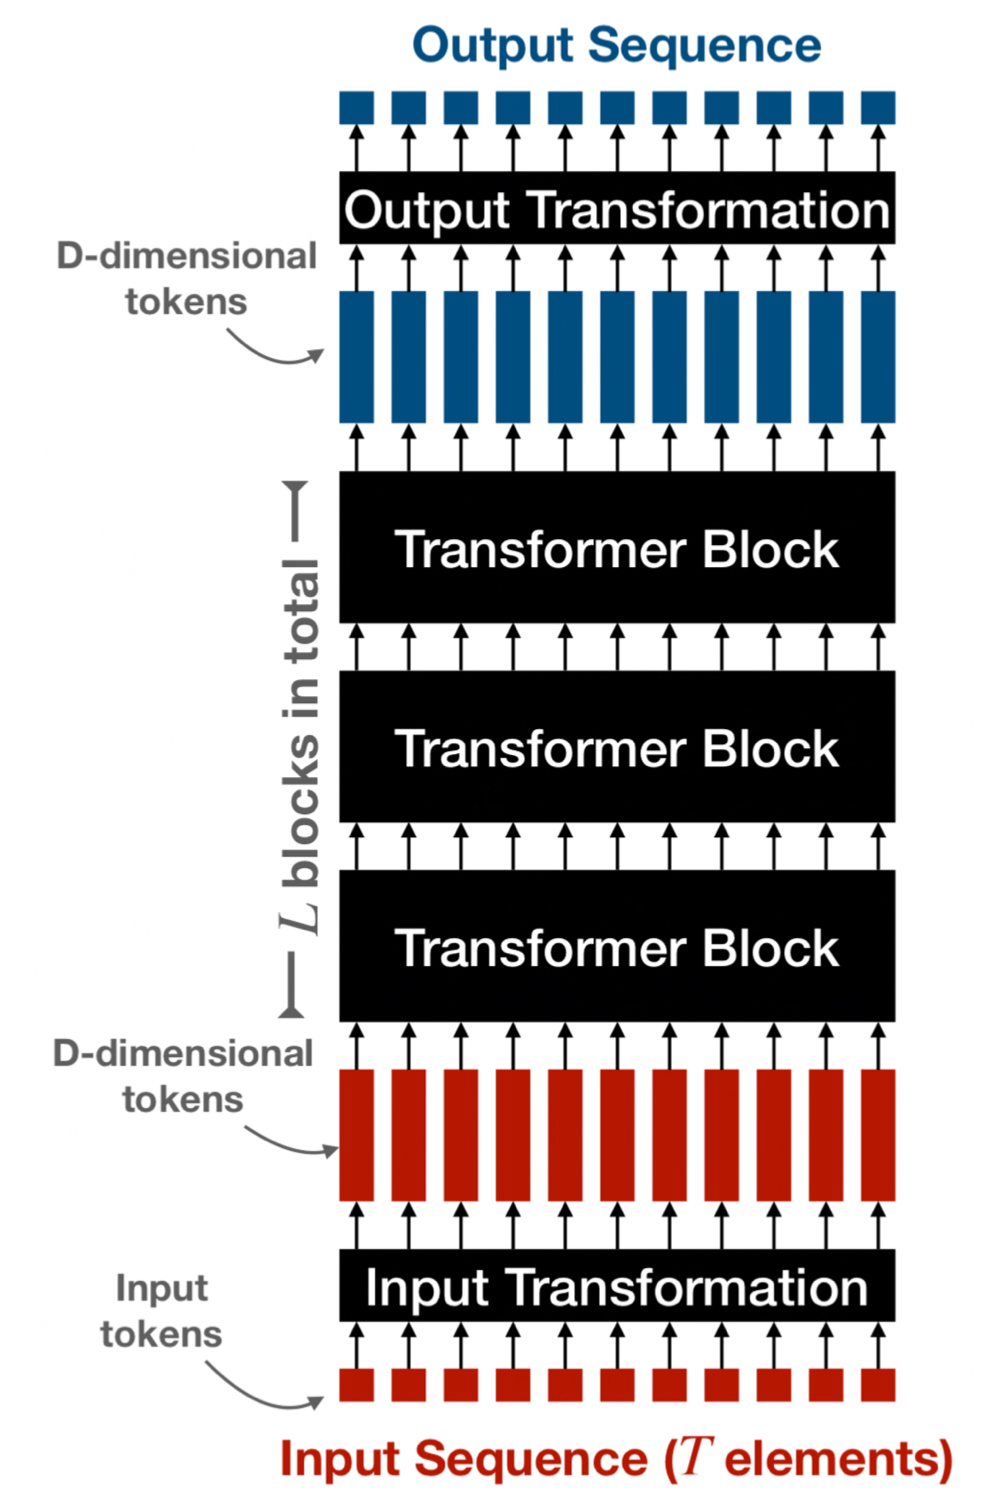
\includegraphics[width=0.4\columnwidth]{figures/transformer_architecture.jpeg}
%     \vspace{-10pt}
% \end{wrapfigure}

- Self-Attention (SA): mixes information between tokens

- Multi-Layer Percep. (MLP): mixes information within each token

- Skip connections are widely used

- Layer normalization (LN) placed at the start of a residual branch

% \begin{wrapfigure}{l}{0.2\columnwidth}
%   % \centering
%   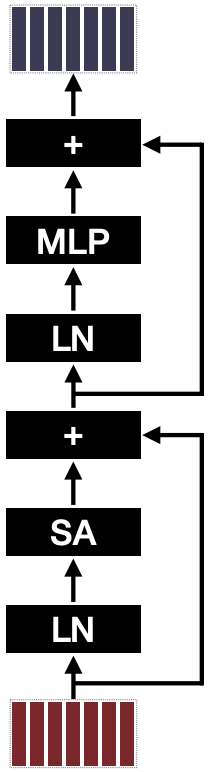
\includegraphics[width=0.2\columnwidth]{figures/transformer_block.png}
% %   \caption{}
% %   \label{fig:cfm_pca2D_wrapped}
% \end{wrapfigure}

\subsection*{Text Token Embeddings}

- Tokenization: split text into sequence of tokens (predefined)

- Convert each token ID $i\in\{1,...,N_{vocab}\}$ into $\mathbf{w}_{i}\in\mathbb{R}^{D}$

- Matrix multiplication $\mathbf{W}\cdot\mathbf{e}_{i}=\mathbf{W}_{:,i}=\mathbf{w}_{i}{\mathrm{~(with~\mathbf{W}\in\mathbb{R}^{D \times N_{vocab}}}})$


- $\mathbf{W}$ learned via backpropagation
% , along with all other transformer parameters (however, the tokenizer procedure is typically fixed in advance and not learned)

- Input sequence of $T$ tokens leads to an input matrix $X\in\mathbb{R}^{T\times D}$

\subsection*{Attention: learning input-dependent weighted average}



% - Attention is a function that transforms a sequence of tokens to a new sequence of tokens using a learned input-dependent weighted average

- Input tokens : $V\in\mathbb{R}^{T_{i n}\times D}$, Output tokens : $Z\in\mathbb{R}^{T_{out}\times D}$

% - Output tokens are simply a weighted average of
% the input tokens:
$z_{i}=\sum_{j=1}^{T_{i}}p_{i j}v_{j}$ i.e. $Z=P V$, Weighting coefficients ${\cal P}\in[0,1]^{T_{out}\times T_{i n}}$ valid probability distributions over input $\textstyle\sum_{j=1}^{T_{i n}}p_{i j}=1$


\begin{wrapfigure}{r}{0.4\columnwidth}
  % \centering
  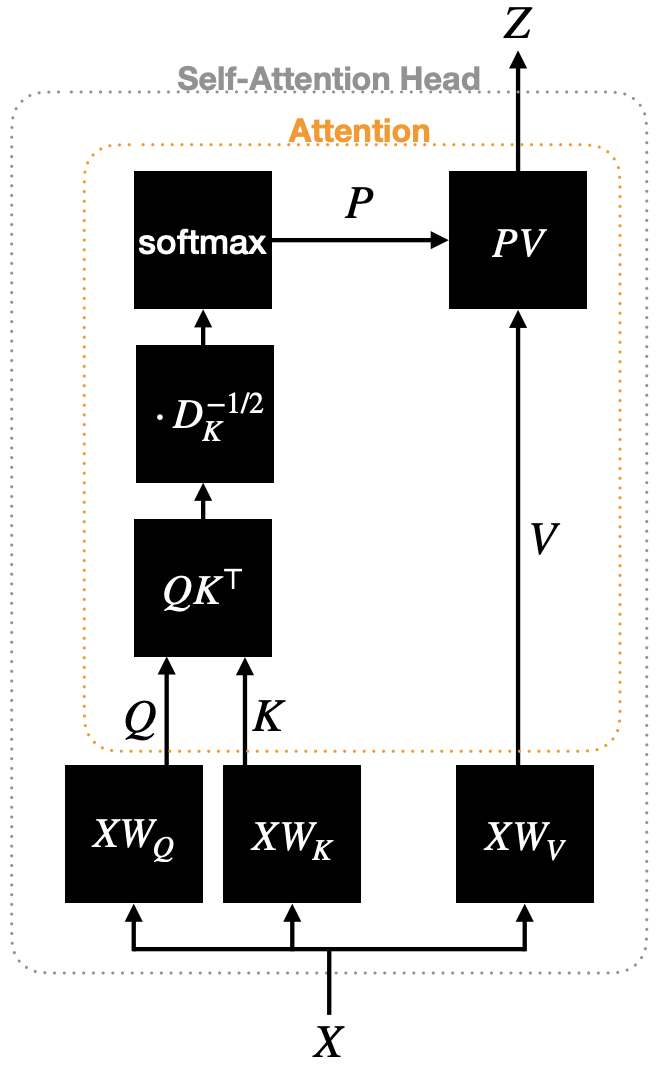
\includegraphics[width=0.4\columnwidth]{figures/self_attention.png}
%   \caption{}
%   \label{fig:cfm_pca2D_wrapped}
\end{wrapfigure}

- Query tokens : $Q\in\mathbb{R}^{T_{out}\times D_{K}}$, Key tokens : $K\in\mathbb{R}^{T_{in}\times D_{K}}$


- Determine weight $p_{i,j}$ based on how simmilar $q_i$ and $k_j$ are.

- Use inner product to obtain raw similarity scores.

- Normalize with softmax (scaled temperature by $\sqrt{D_{K}}$) to obtain a probability distribution. (applied on each row independently)

% - $P=\mathrm{softmax}\left({\frac{Q K^{\mathsf{T}}}{\sqrt{D_{K}}}}\right)$ 
% - The softmax is applied on each row independently. 

- Scaling $\rightarrow$ uniformity at initialization and faster convergence

\subsection*{Self-Attention}



- $V,K,Q$ all derived from same input token
sequence $X\in\mathbb{R}^{T\times D}$

- Values : $V=X W_{V}\in\mathbb{R}^{T\times D},\,W_{V}\in\mathbb{R}^{D\times D}$

- Keys : $K=X W_{K}\in\mathbb{R}^{T\times D_{K}},\,W_{K}\in\mathbb{R}^{D\times D_{K}}$

- Queries : $Q=X W_{Q}\in\mathbb{R}^{T\times D_{K}},W_{Q}\in\mathbb{R}^{D\times D_{K}}$

- $W_{Q},\,W_{V},\,W_{K}$ are learned params.

- $Z=\mathrm{softmax}\left(\frac{X W_{Q}W_{K}^{T}X^{T}}{\sqrt{D_{K}}}\right)X W_{V}$

\subsubsection*{Multi-Head Self-Attention}

% \begin{wrapfigure}{r}{0.3\columnwidth} 
%   \centering
%   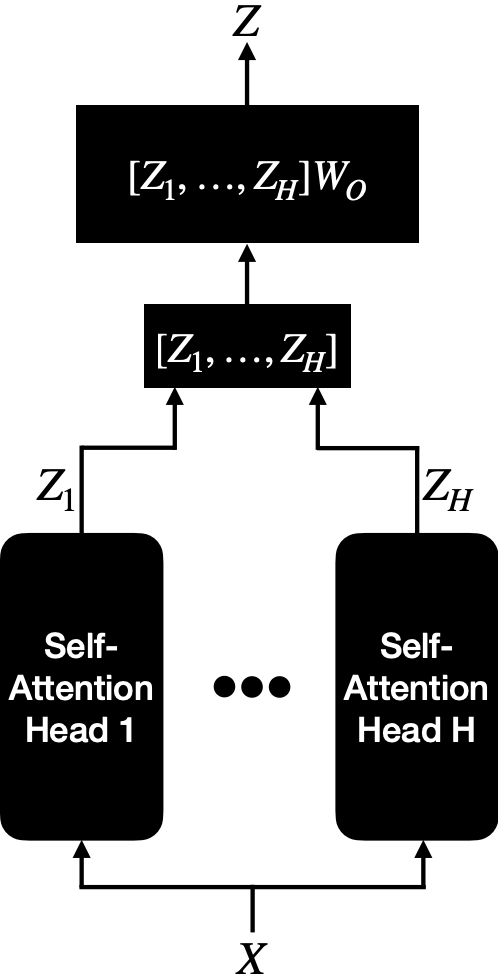
\includegraphics[width=0.3\columnwidth]{figures/multi_head.png}
% \end{wrapfigure}

- Run $H$ Self-Attention “heads” in parallel 
$Z_{h}={\mathrm{softmax}}\left({\frac{X W_{Q,h}W_{K,h}^{\mathsf{T}}X^{\mathsf{T}}}{\sqrt{D_{K}}}}\right)X W_{V,h}\in\mathbb{R}^{T\times D_{V}}$, 
$W_{V,h}\in\mathbb{R}^{D\times D_{V}},\,W_{K,h}\in\mathbb{R}^{D\times D_{K}},\,W_{Q,h}\in\mathbb{R}^{D\times D_{K}}$,
$Z=[Z_{1},\dots,Z_{H}]W_{o}$ where $W_{O}\in\mathbb{R}^{H D_{V}\times D}$ is learned via backprop
% \lipsum[1]

\subsection*{Positional Information}

- Attention by itself does not account for the order of input

- positional encoding in the network $p o s:\left\{1,...,T\right\}\rightarrow\mathbb{R}^{D}$

- e.g. $W_{p o s}$ corresponding to each token's position $t$ to the input embedding. $W_{p o s}\in\mathbb{R}^{D\times T}$ is learned via backprop

\subsection*{MLP: Mixing Information within Tokens}
- Apply the same transformation to each token
independently: $M L P(X)=\varphi(X W_{1})W_{2}$,
$W_{1},W_{2}\in\mathbb{R}^{D\times D}$ learned via backprop

\subsection*{Output Transformations}

% - typically simple: linear transformation or a small MLP

- Single output: transfo. to a special taskspecific input token or to the average tks. Multi outputs: transfo to each token indep.

\subsection*{Vision Transformer Architecture}

% - Self-attention, more general than convolution 

- The receptive field is the whole image after one SA layer

- ViTs require more data than CNNs, reduced inductive bias in extracting local features

- Model attends to image regions semantically relevant for clf

\subsection*{Encoders \& Decoders}

% \begin{wrapfigure}{r}{0.3\columnwidth} 
%   \centering
%   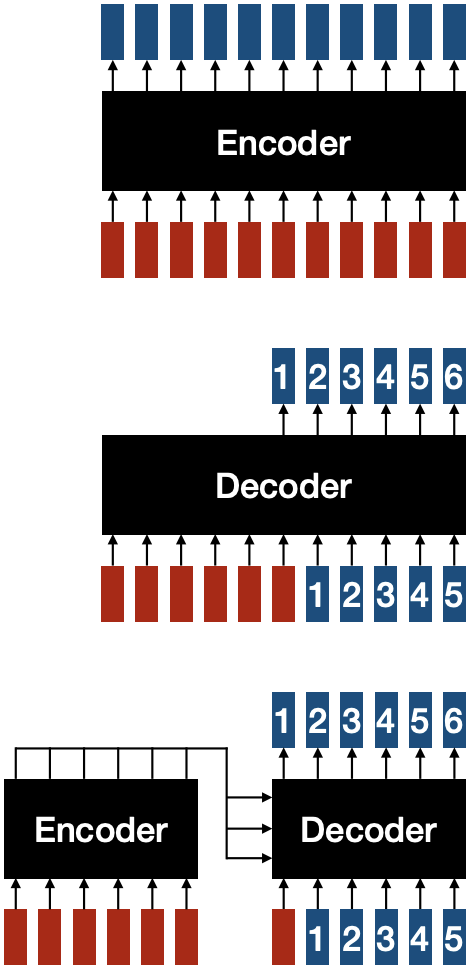
\includegraphics[width=0.3\columnwidth]{figures/encoders_decoders.png}
% \end{wrapfigure}

- Encoders: fixed output size and process all inputs simultaneously

- Decoders: Auto-regressively sample the next token as $x_{t+1}\sim s o f i m a x(f(x_{1},....,x_{t}))$
%  and use it as new input token. Capable of generating responses of arbitrary length.

% - Encoder-decoder (e.g., translation): First encode the whole input (e.g., in one language) and then decode to token by token (e.g., in a different language)

\sectiondivider

\sectionnewcolor
\section*{Adversarial ML}

- We don't understand how NN models generalize and react to shifts in the distribution of data (i.e., distribution shifts)

- Classification problem: $(X,Y)\sim{\mathcal{D}},\;Y$ with range $\{-1,1\}$

- Standard risk: average zero-one loss over $X$: $R(f)=\mathbb{E}_{\mathcal{D}}\left[1_{f(X)\neq Y}\right]=\mathbb{P}_{\mathcal{D}}\left[f(X)\neq Y\right]$ i.e. minimise proba of wrong prediction.


- Adversarial risk: average zero-one loss over small, worst-case perturbations of $X$: $R_{\varepsilon}(f)={{{\mathbb{E}}}}_{\mathcal{D}}\left[\operatorname*{max}_{\hat{x},\|\hat{x}-X\|\leq\varepsilon}1_{f(\hat{x})\neq Y}\right]$

\subsection*{Generating adversarial examples}

- Task: given an input $(x, y)$ and a model $f : \mathcal{X}\rightarrow \{-1,1\}$ find an input $\hat{x}$ s.t.: 
a) $\|{\hat{x}}-x\|\leq\varepsilon$ b) the model $f$ makes a mistake on it.

- Trivial case: x already missclassified $\rightarrow$ no action required

- General case: ${\mathrm{find~}}{\hat{x}}~\mathrm{such~that}{\mathrm{~at}}f({\hat{x}})\neq y\operatorname{and}{\big\vert\vert}{\hat{x}}-x\vert\vert\leq\varepsilon$ i.e. $\hat{x}\in B_{x}(\varepsilon)\cap\{x^{\prime}f(x^{\prime})=-\,y\}$

- Optimization problem with respect to the inputs

- Problem: optimizing the indicator function is difficult: 1) The indicator function $1$ is not continuous 2) The NN prediction $f$ outputs discrete class values $\{-1,1\}$

- Replace the difficult problem involving the indicator with a smooth problem $\operatorname*{max}_{\hat{x},\|\hat{x}-X\|\leq\varepsilon}1_{f(\hat{x})\neq Y} \rightarrow \operatorname*{max}_{\hat{x},\|\hat{x}-X\|\leq\varepsilon}\ell(yg(\hat{x}))$

\begin{wrapfigure}{r}{0.5\columnwidth} 
    \centering
    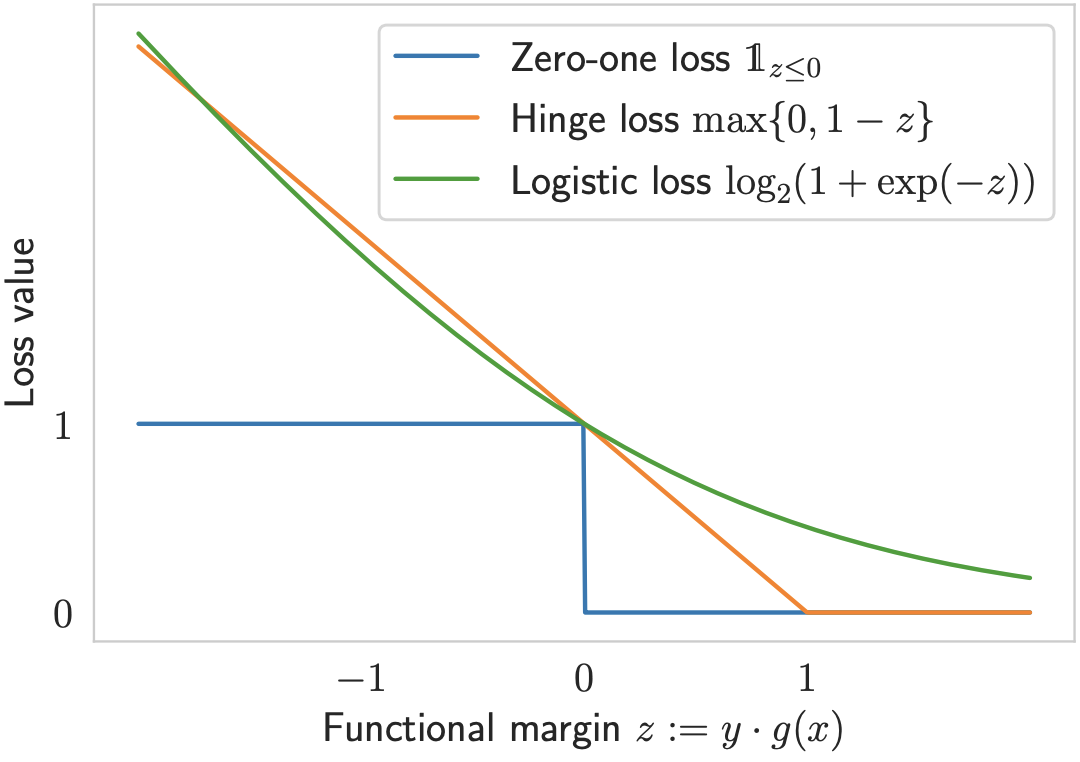
\includegraphics[width=0.5\columnwidth]{figures/classification_losses.png}
\end{wrapfigure}
- decreasing, margin-based (i.e., dependent on $y * g(x)$) classification losses

\subsection*{White-Box attacks}

- Solve $\operatorname*{max}_{\hat{x},\|\hat{x}-X\|\leq\varepsilon}\ell(yg(\hat{x}))$ knowing $g$

- $\nabla_{x}{\ell}(y g(x))=y\ell^{\prime}(y g(x))\,\nabla_{x}g(x)$, with $y\ell^{\prime}(y g(x)) \leq 0$ since classification losses are decreasing.

- Move in direction of $\propto-\,y\,\nabla_{x}g(x)$

- Interpretation $f(x)=\mathrm{{sign}}(g(x))$: If $y=1$ we want to decrease $g(x)$ and follow $-\nabla_{x}g(x)$. If $y=-1$ we want to decrease $g(x)$ and follow $\nabla_{x}g(x)$

- By using $\ell$ and not directly $yg(\hat{x})$ it will extend to multi-class classification and robust training.

- linearize the loss $\tilde{\ell}(x):={\ell}(y g(x))$

$\operatorname*{max}_{\|{\hat{x}}-x\|\leq\varepsilon}{\tilde{\ell}}(x)\\\approx\operatorname*{max}_{\|{\hat{x}}-x\|\leq\varepsilon}{\tilde{\ell}}(x)+\nabla_{x}{\tilde{\ell}}(x)^{T}({\hat{x}}-x) \\={\tilde{\ell}}(x)+\operatorname*{max}_{\|{\hat{x}}-x\|\leq\varepsilon}{\nabla}_{x}{\tilde{\ell}}(x)^{T}({\hat{x}}-x) \\={\tilde{\ell}}(x)+\operatorname*{max}_{\|\delta\|\leq\varepsilon}{\nabla}_{x}{\tilde{\ell}}(x)^{T}{\delta}$

- We need to maximize the inner product under a norm constraint, i.e. find the optimal local update

- This is a simple problem for which we can get a closed-form solution depending on the norm used to measure the perturbation size $||\delta||$

\subsubsection*{One-step attack}

- Solution for the $\ell_2$ norm:

$\delta_{2}^{\star}=\varepsilon\cdot\frac{\nabla_{x}\tilde{\ell}(x)}{||\nabla_{x}\tilde{\ell}(x)||_{2}}=-\;\varepsilon y*\frac{\nabla_{x}g(x)}{||\nabla_{x}g(x)||_{2}} \Rightarrow \\ \hat{x}=x-\varepsilon y\cdot\frac{\nabla_{x}g(x)}{\|\nabla_{x}g(x)\|_{2}}$

- Solution for the $\ell_{\infty}$ norm called \textbf{Fast Gradient Sign Method}:

$\delta_{\infty}^{\star}=\varepsilon\cdot\mathrm{sign}(\nabla_{x}\tilde{\ell}(x))=-\,\varepsilon y\cdot\mathrm{sign}(\nabla_{x}g(x)) \Rightarrow \\ {\hat{x}}=x-\varepsilon y\cdot\operatorname{sign}(\nabla_{x}g(x))$

\subsubsection*{Multi-step attack}


- These updates can be done iteratively and combined with a projection $\Pi$ on the feasible set (i.e., balls $\ell_2$ / $\ell_\infty$ here)

- Projected Gradient Descent (PGD attack)

- $\ell_2$ norm:

$\delta^{t+1}=\Pi_{B_{2}(e)} [\delta^{t}+\alpha\cdot\frac{\nabla\tilde{\ell}(x+\delta^{t})}{\|\nabla\tilde{\ell}(x+\delta^{t})\|_{2}}]$

$\Pi_{B_{2}(\varepsilon)}(\delta)=\left\{\begin{array}{l l}{\varepsilon\cdot\delta/\|\delta\|_{2},\quad{\mathrm{if~}}\|\delta\|_{2}\geq\varepsilon}\\ {\delta \mathrm{~otherwise}}\end{array}\right.$

- $\ell_\infty$ norm:

$\delta^{t+1}=\Pi_{B_{\infty}(\varepsilon)}\left[\delta^{t}+\alpha\cdot\mathrm{sign}(\nabla\tilde{\ell}(x+\delta^{t}))\right],$

$\Pi_{B_{\infty}(\varepsilon)}(\delta)_i=\left\{\begin{array}{l l}{\varepsilon\cdot\mathrm{sign}(\delta_{i}),\ \ \ \mathrm{if}\ |\delta_{i}|\geq\varepsilon}\\ {\delta_i \mathrm{~otherwise}}\end{array}\right.$

- the gradients are computed by backprop w.r.t. inputs, not parameters!

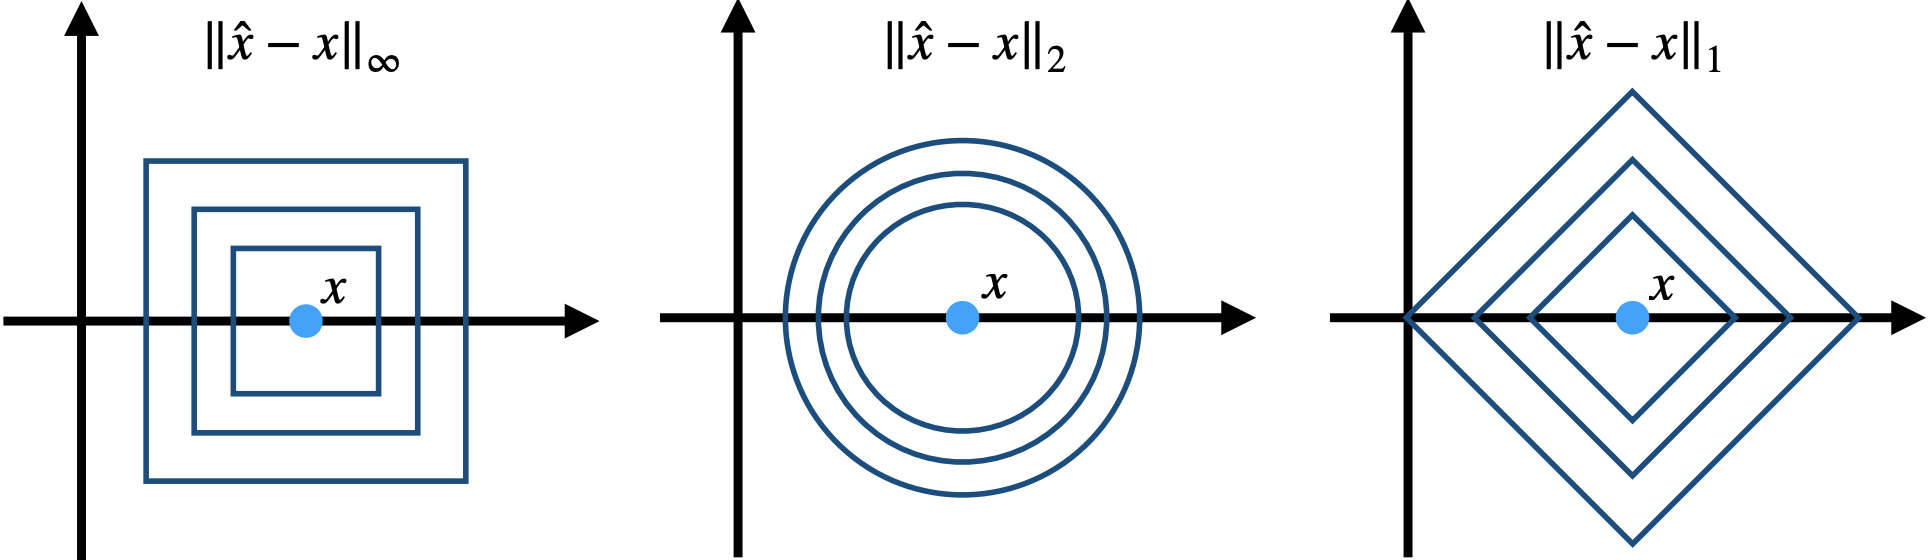
\includegraphics[width=\columnwidth]{figures/lp_norms.png}

\subsection*{Black-box attacks}

- We don't know $g(x)$

- Obtaining a surrogate model can be costly and there is no guarantee of success

- Query-based methods often require a lot of queries (10k-100k), easy to restrict access for the attacker!

\subsubsection*{Query-based gradient estimation}

- Score-based: we can query the continuous model scores $g(x)\in \mathbb{R}$. We can approximate the gradient by using the finite difference formula:

$\nabla_{x}g(x)\approx\sum_{i=1}^{d}\frac{g(x+\alpha e_{i})-g(x)}{\alpha}e_{i}$

- Decision-based: we can query only the predicted class $f(x) \in \{-1,1\}$, similar techniques can be adapted for the decision-based case.

\subsubsection*{Transfer Attacks}

- Train a similar surrogate model ${\hat{f}}\approx f$ on similar data

- Model stealing (query $f$ given some unlabeled inputs $\{x_{n},f(x_{n})\}_{n=1}^{N}$) can facilitate transfer attacks.


\subsection*{Adversarial training}

- Adversarial training: the goal is to minimize the adversarial risk:

$\operatorname*{min}_{\theta}R_{\varepsilon}(f_{\theta})=\mathbb{E}_{\mathcal{D}}\left[\operatorname*{max}_{\hat{x},\|\hat{x}-X\|\leq\varepsilon}1_{f(\hat{x})\neq Y}\right]$

- $\mathcal{D}$ unknown $\rightarrow$ approximate it with a sample average + classification loss is non-continuous $\rightarrow$ use a smooth loss $\Rightarrow$

$\operatorname*{min}_{\theta}{\frac{1}{N}}\sum_{n=1}^{N} \operatorname*{max}_{\hat{x}_{n},\|x_{n}-\hat{x}_{n}\|\leq\varepsilon}{\ell}(y_{n}g_{\theta}(\hat{x}_{n}))$

1) $\forall x_n\;, \hat{x}_{n}^{\star}\approx\arg\operatorname*{max}_{||x_{n}-\hat{x}_{n}|\leq\varepsilon}\ell(y_{n}g_{\theta}(\hat{x}_{n}))$

2) GD step w.r.t. $\theta$ using $\frac{1}{N}\sum_{n=1}^{N}\nabla_{\theta}{\ell}(y_{n}g_{\theta}({\hat{x}}_{n}^{\star}))$

\subsubsection*{Advantages}

- state-of-the-art approach for robust classification

- more interpretable gradients

- fully compatible with SGD

\subsubsection*{Disadvantages}

- Increased computational time: proportional to the number of PGD steps

- Robustness-accuracy tradeoff: using too large $\varepsilon$ leads to worse standard accuracy

\subsubsection*{Adversarial Example}
% \begin{wrapfigure}{r}{0.5\columnwidth} 
%     \centering
%     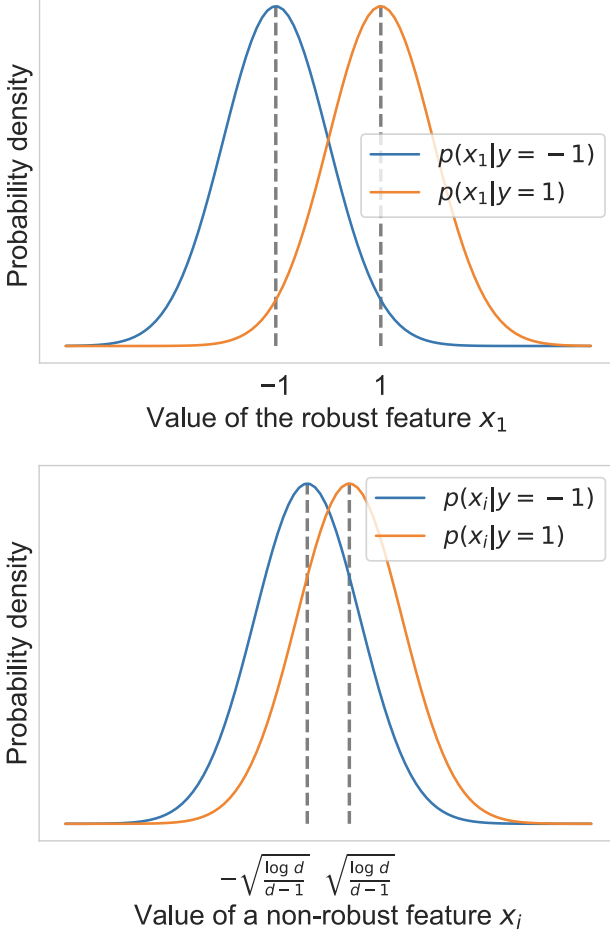
\includegraphics[width=0.5\columnwidth]{figures/adversarial_example.png}
% \end{wrapfigure}

$x\in\mathbb{R}^{d},y\sim{{Bernoulli}}(\{-1,1\}),Z_{i}\sim{\mathcal{N}}(0,1)$

- Robust features: $x_{1}=y+Z_{1}$

- Non-robust features: $x_{i}=y{\sqrt{\frac{\log d}{d-1}}}+Z_{i}, \; \forall i \in \{-1, 1\}$

- $d\to\infty \Rightarrow \ \uparrow$ adversarial risk and $\downarrow$ standard risk 

- using the robust feature $x_1$:

MLE: $\arg\operatorname*{max}_{\hat{y}\in\{\pm1\}}p(\hat{y}\;\vert\;x_{1})
=\\\operatorname*{arg}\operatorname*{max}_{{\hat{y}}\in\{\pm1\}}{\frac{p(x_{1}\mid{\hat{y}})p({\hat{y}})}{p(x_{1})}}
=\operatorname*{arg}\operatorname*{max}_{{\hat{y}}\in\{\pm1\}}{p(x_{1}\mid{\hat{y}})}$ 
assuming $p(y=1)=p(y=-1)$

- Standard Risk: $\int_{0}^{\infty}{\frac{1}{\sqrt{2\pi}}}e^{-0.5(x+1)^{2}}d x\approx0.16$ good but not perfect!

- using both robust and non-robust features:

MLE for all features $x_{i}=y a_{i}+Z_{i}$

$\arg\operatorname*{max}_{{\hat{y}}\in\{\pm1\}}p({\hat{y}}\mid x)$

$=\arg\operatorname*{max}_{{\hat{y}}\in\{\pm1\}}\prod_{i=1}^{d}p(x_{i}\mid{\hat{y}})$

$=\arg\operatorname*{max}_{{\hat{y}}\in\{\pm1\}}\sum_{i=1}^{d}\log p(x_{i}\mid{\hat{y}})$

$=\arg\operatorname*{max}_{{\hat{y}}\in\{\pm1\}}\sum_{i=1}^{d}\log \frac{1}{\sqrt{2\pi}}e^{-\frac{1}{2}(x_{i}-\hat{y}a_{i})^{2}}$

$=\arg\operatorname*{min}_{{\hat{y}}\in\{\pm1\}}\sum_{i=1}^{d}(x_{i}-\hat{y}a_{i})^{2}$

$=\arg\operatorname*{min}_{{\hat{y}}\in\{\pm1\}}\sum_{i=1}^{d}(x_{i}^{2}-2x_{i}\hat{y}a_{i}+\hat{y}^{2}a_{i}^{2})$

$=\arg\operatorname*{max}_{\hat{y}\in\{\pm1\}}{\hat{y}}\sum_{i=1}^{d}x_{i}a_{i}$

${\hat{y}}\sum_{i=1}^{d}x_{i}a_{i}=\hat{y}y(\sum_{i=1}^{d}a_{i}^{2})+\hat{y}\sum_{i=1}^{d}a_{i}Z_{i}=\hat{y}y(1+\log(d))+\hat{y}Z$ where $Z:=\textstyle\sum_{i=1}^{d}a_{i}Z_{i}\sim{\mathcal{N}}(0,1+\log d)$

Scaling by $1/(1+\log d)$ the MLE results in:

$y{\hat{y}}+{\hat{y}}Z\operatorname{with}Z\sim{\mathcal{N}}(0,1/(1+\log d))$

$d\rightarrow\infty,{\hat{y}}Z\rightarrow0 \Rightarrow$ standard risk $R(f) \rightarrow 0$ 

- using the non-robust features improves standard risk!

- Adversarial risk:

The adversary can use tiny $\ell_\infty$ perturbations:

$\varepsilon=2\sqrt{\frac{\log d}{d-1}}\,(\to0\,\mathrm{when})\,d\to\infty)$

${\hat{x}}_{1}=\left(1-2\sqrt{\frac{\log d}{d-1}}\right)y+Z_{1}$, almost unaffected

$\hat{x}_{i}=-\sqrt{\frac{\log d}{d-1}}y+Z_{i}$, completely flipped

$R_{\varepsilon}(f) \approx 1 \Rightarrow$ tradeoff between accuracy and robustness.

\sectiondivider

\sectionnewcolor
\section{Matrix Factorization}

Given items (movies) $d=1, 2, . . . , D$ and users $n= 1, 2, . . . , N$, we define X to be the $D \times N$ matrix containing all rating entries. That is, $x_{dn}$ is the rating of n-th user for d-th item.
Note that most ratings $x_{dn}$ are missing, and our task is to predict them accurately.

\subsection*{Algorithm}

$X \approx WZ^T$, $W \in \mathbb{R}^{D \times K}, \ Z \in \mathbb{R}^{N \times K}$ tall matrices $K << N, D$

$\operatorname*{min}_{W,Z}~{\mathcal{L}}(W,Z):=\frac{1}{2}\sum_{(d,n)\in\mathbb{Q}} [x_{dn}-(WZ^T)_{dn}]^2$

- We hope to ``explain" each rating $x_{dn}$ by a numerical representation of the corresponding item and user - in fact by the inner product of an item feature vector with the user feature vector.



- The set $\Omega\subseteq\left[D\right]\times\left[N\right]$ collects the indices of the observed ratings of the input matrix $X$.

- This cost is not jointly convex w.r.t. W and Z, nor identifiable as $(w^*, z^*) \Leftrightarrow (\beta w^*, \beta^{-1} z^*)$

\subsection*{Choosing K}

- $\uparrow K \Rightarrow$ overfitting ($\Leftrightarrow \ \downarrow K \Rightarrow$ underfitting). 
For $K >> N,D \Rightarrow (W^*, Z^{*^T}) = (X, I) = (I, X)$

\subsection*{Regularization}

$\frac{1}{2}\sum_{(d,n)\in\Omega}[x_{d n}-(W Z^{T})_{d n}]^{2}+\frac{\lambda_{w}}{2}||{W}||_{\mathrm{Frob}}^{2}+\frac{\lambda_{z}}{2}||{Z}||_{\mathrm{Frob}}^{2}$
$\lambda_{w},\lambda_{z}\, \in \mathbb{R} > 0$


\subsection*{Stochastic Gradient Descent}

$\mathcal{L} = \frac{1}{|\Omega|} \sum_{(d,n)\in\Omega}\underbrace{{\frac{1}{2}}[x_{d n}-(\mathbf{W}\mathbf{Z}^{\textsf{T}})_{d n}]^{2}}_{f_{d,n}}$

For one fixed element (d, n) of the sum, we derive the gradient entry (d', k) for W:

${\frac{\partial}{\partial w_{d^{\prime},k}}}f_{d,n}(W, Z) \in \mathbb{R}^{D\times K}=\\\left\{\begin{array}{l l}{-\left[x_{d n}-({\bf W Z}^{T})_{d n}\right]z_{n,k}\;\;\;\mathrm{if}\;d^{\prime}=d} \\ {0 \mathrm{~otherwise}}\end{array}\right.$

${\frac{\partial}{\partial z_{n^{\prime},k}}}f_{d,n}(W, Z)\in \mathbb{R}^{N\times K}=\\\left\{\begin{array}{l l}{-\left[x_{d n}-({\bf W Z}^{T})_{d n}\right]w_{d,k}\;\;\;\mathrm{if}\;n^{\prime}=n} \\ {0 \mathrm{~otherwise}}\end{array}\right.$

- cost: $\Theta(K)$ which is cheap!

\subsection*{Alternating Least Squares}

- No missing entries:

${\textstyle\frac{1}{2}}\sum_{d=1}^{D}\sum_{n=1}^{N}\left[x_{d n}-\left(W\mathbf{Z}^{\mathsf{T}}\right)_{d n}\right]^{2}$
$\\=\frac{1}{2}\|\mathbf{X}-\mathbf{W}\mathbf{Z}^{\mathsf{T}}\|_{{Frob}}^{2}$

- We first minimize w.r.t. Z for fixed W and then minimize W given Z (closed form solutions):

$Z^{\mathsf{T}}:=(\mathsf{W}^{\mathsf{T}}\mathsf{W}+\lambda_{z}\mathsf{I}_{K})^{-1}\mathsf{W}^{\mathsf{T}}\mathsf{X}$

$\mathbf{W}^{\mathsf{T}}:=(\mathbf{Z}^{\mathsf{T}}\mathbf{Z}+\lambda_{w}\mathbf{I}_{K})^{-1}\mathbf{Z}^{\mathsf{T}}\mathbf{X}^{\mathsf{T}}$

- Cost: need to invert a $K \times K$ matrix

- With missing entries:
Can you derive the ALS updates for the more general setting, when only the ratings $(d, n) \in \Omega$ contribute to the cost, i.e.
$\frac{1}{2}\sum_{(d,n)\in\Omega}\big[x_{d n}-\big(\mathsf{W Z}^{\mathsf{T}}\big)_{d n}\big]^{2}$

Compute the gradient with respect to each group of variables, and set to zero.

% \subsection*{Update for $Z$ with fixed $W$:}
% The ALS update for $Z^{\mathsf{T}}$ is given by:
% \[
% Z^{\mathsf{T}} := \left(W^{\mathsf{T}}W + \lambda_{z}I_{K}\right)^{-1}W^{\mathsf{T}}X
% \]
% For each $(n, k)$ where $(d', n) \in \Omega$, the update for the $k$-th component of $Z^{\mathsf{T}}$ is:
% \[
% \left(Z^{\mathsf{T}}\right)_{n,k} := \left(\sum_{d':(d',n)\in\Omega} w_{d',k'}w_{d',k} + \lambda_{z}\delta_{k,k'}\right)^{-1} \sum_{d':(d',n)\in\Omega} w_{d',k'}x_{d',n}
% \]

% \subsection*{Update for $W$ with fixed $Z$:}
% The ALS update for $W^{\mathsf{T}}$ is given by:
% \[
% W^{\mathsf{T}} := \left(Z^{\mathsf{T}}Z + \lambda_{w}I_{K}\right)^{-1}Z^{\mathsf{T}}X^{\mathsf{T}}
% \]
% For each $(d, k)$ where $(d, n') \in \Omega$, the update for the $k$-th component of $W^{\mathsf{T}}$ is:
% \[
% \left(W^{\mathsf{T}}\right)_{d,k} := \left(\sum_{n':(d,n')\in\Omega} z_{n',k'}z_{n',k} + \lambda_{w}\delta_{k,k'}\right)^{-1} \sum_{n':(d,n')\in\Omega} z_{n',k'}x_{d,n'}
% \]

\sectiondivider

\sectionnewcolor
\section*{Text Representation}

-Finding numerical representations for words is fundamental for all machine learning methods dealing with text data.

-Goal: For each word, find mapping (embedding) $w_{i} \mapsto \mathbf{w}_{i} \in \mathbb{R}^{K}$

\subsection*{Co-Occurence Matrix}

-A big corpus of un-labeled text can be represented as the co-occurrence counts. $n_{i j}:=$ \#contexts where word $w_{i}$ occurs together with word $w_{j}$.

- Needs definition of Context e.g. document, paragraph, sentence, window and Vocabulary $\mathcal{V}:=\left\{w_{1}, \ldots, w_{D}\right\}$

- For words $w_{d}=1,2, \ldots, D$ and context words $w_{n}=1,2, \ldots, N$, the co-occurence counts $n_{i j}$ form a very sparse $D \times N$ matrix.

\subsection*{Learning Word-Representations}

- Find a factorization of the cooccurence matrix!

- Typically uses $\log$ of the actual counts, i.e. $x_{d n}:=\log \left(n_{d n}\right)$.

- Aim to find $\mathbf{W}, \mathbf{Z}$ s.t. $
\mathbf{X} \approx \mathbf{W} \mathbf{Z}^{\top}
$

$
\min _{\mathbf{W}, \mathbf{Z}} \mathcal{L}(\mathbf{W}, \mathbf{Z}):=\\\frac{1}{2} \sum_{(d, n) \in \Omega} f_{d n}\left[x_{d n}-\left(\mathbf{W} \mathbf{Z}^{\top}\right) d n\right]^{2}
$

where $\mathbf{W} \in \mathbb{R}^{D \times K}$, $\mathbf{Z} \in \mathbb{R}^{N \times K}$, $K \ll$ $D, N$, $\Omega \subseteq[D] \times[N]$ indices of non-zeros of the count matrix $\mathbf{X}$, $f_{d n}$ are weights to each entry.

\subsection*{GloVe}
A variant of word2vec.

$f_{d n}:=\min \left\{1,\left(n_{d n} / n_{\max }\right)^{\alpha}\right\}, \quad \alpha \in[0 ; 1] \quad$ (e.g. $\alpha=\frac{3}{4}$)

\textbf{Note:} Choosing K; $K$ e.g. 50, 100, 500

\subsection*{Training}
- Stochastic Gradient Descent (SGD) ($\Theta(K)$ per step $\rightarrow$ easily parralelizable)

- Alternating Least-Squares (ALS)

\subsection*{Skip-Gram Model}
- Uses binary classification (logistic regression objective), to separate real word pairs $\left(w_{d}, w_{n}\right)$ from fake word pairs. Same inner product score $=$ matrix factorization.

- Given $w_{d}$, a context word $w_{n}$ is:

real $=$ appearing together in a context window of size 5

fake $=$ any word $w_{n^{\prime}}$ sampled randomly: Negative sampling (also: Noise Contrastive Estimation)

\section*{Learning Representations of Sentences \& Documents}
- Supervised: For a supervised task (e.g. predicting the emotion of a tweet), we can use matrix factorization or CNNs.
- Unsupervised: 

Adding or averaging (fixed, given) word vectors, 

Training word vectors such that adding/averaging works well

Direct unsupervised training for sentences (appearing together with context sentences) instead of words

\subsection*{Fast Text}
Matrix factorization to learn document/sentence representations (supervised).

Given a sentence $s_{n}=$ $\left(w_{1}, w_{2}, \ldots, w_{m}\right)$, let $\mathbf{x}_{n} \in \mathbb{R}^{|\mathcal{V}|}$ be the bag-of-words representation of the sentence.

$$
\min _{\mathbf{W}, \mathbf{Z}} \mathcal{L}(\mathbf{W}, \mathbf{Z}):=\sum_{s_{n} \text { a sentence }} f\left(y_{n} \mathbf{W} \mathbf{Z}^{\top} \mathbf{x}_{n}\right)
$$

where $\mathbf{W} \in \mathbb{R}^{1 \times K}, \mathbf{Z} \in \mathbb{R}^{|\mathcal{V}| \times K}$ are the variables, and the vector $\mathbf{x}_{n} \in \mathbb{R}^{|\mathcal{V}|}$ represents our $n$-th training sentence.

Here $f$ is a linear classifier loss function, and $y_{n} \in\{ \pm 1\}$ is the classification label for sentence $\mathbf{x}_{n}$.


\subsection*{Language Models}
\subsubsection*{Selfsupervised training:}
- Can a model generate text? train classifier to predict the continuation (next word) of given text

- Multi-class:
Use soft-max loss function with a large number of classes $D=$ vocabulary size

- Binary classification: 
Predict if next word is real or fake (i.e. as in word2vec)

- Impressive recent progress using large models, such as transformers

\sectiondivider

\sectionnewcolor
\newpage
\section{{\textcolor[RGB]{255,0,0}{This is RGB red text.}}}

For $x \in[r_{i-1},r_{i}]$ \\
$r(x)={\tilde{a}}_{1}x+{\tilde{b}}_{1}+\sum_{j=2}^{m}{\tilde{a}}_{j}(x-{\tilde{b}}_{j})_{+}$

\hrulefill

$\begin{array}{l}{{\mathsf{For}\;x\in[r_{i-1},r_{i}]}}\\ {{r(x)={\tilde{a}}_{1}x+{\tilde{b}}_{1}+\sum_{j=2}^{m}{\tilde{a}}_{j}(x-{\tilde{b}}_{j})_{+}}}\end{array}$\\
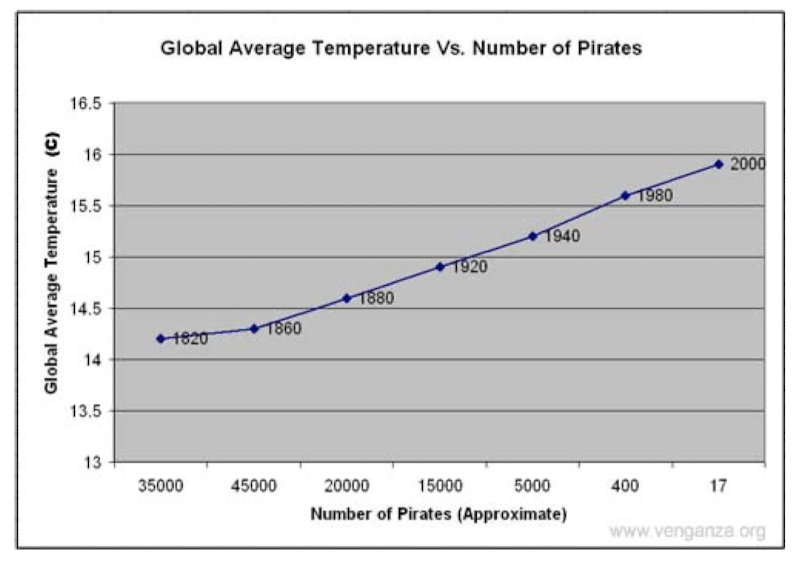
\includegraphics[width=\linewidth]{test_image}

\lipsum[1]

\noindent\dotfill

\lipsum[1]
\sectiondivider

\end{multicols*}

\end{document}
